% !TEX root = handbook-physics.tex
%!TEX TS-program = pdflatex
%!TEX encoding = UTF-8 Unicode






\chapter{Electric Field Potential}
\label{ch-16}
\zhtitle{电场的电势}

\section[Work in Moving Electric Charge]{Work Done in Moving an Electric Charge in an Electrostatic Field}
\label{sec-16.1}
\zhtitle{静电场中移动电荷时所做的功}

\subsection{}\label{16.1.1} The work done in moving an electric charge $q'$ in an electrostatic field of strength $\vb{E}$ \ssect{15.1.3} is independent of the shape of the path along which the charge is moved; it depends only upon the initial and final positions of the charge. In other words, electrostatic forces, like gravitational forces, are potential (conservative) forces \ssect{3.1.6}. The work $\delta W$	 done by the force $\vb{F} = q'\, \vb{E}$ exerted on charge $q'$ in moving it over the distance $\dd \vb{l}$, is equal to:
\zhpar{在场强为 $\vb{E}$ 的静电场中（\ssect{15.1.3}）移动电荷 $q'$ 时所做的功与电荷所经路径的形状无关，只取决于电荷的初始位置和终止位置。换言之，静电力与引力一样，属于有势力（即保守力）（\ssect{3.1.6}）。作用于电荷 $q'$ 的力 $\vb{F} = q'\, \vb{E}$ 使电荷沿位移 $\dd \vb{l}$ 移动时所做的功 $\delta W$ 为：}
\begin{equation*}%
\delta W = F \, \, \dd l \cos \varphi = q' E \cos \alpha\, \dd l,
\end{equation*}
where $\alpha$ is the angle between the directions of vectors $\vb{E}$ and $\dd \vb{l}$, and $\varphi $ is the angle between the directions of the vectors $\vb{F}$ and $\dd \vb{l}$. The work done in a finite movement of charge $q'$ from point $a$ to point $b$ is equal to
\zhpar{式中 $\alpha$ 为矢量 $\vb{E}$ 与 $\dd \vb{l}$ 方向之间的夹角，$\varphi$ 为矢量 $\vb{F}$ 与 $\dd \vb{l}$ 方向之间的夹角。电荷 $q'$ 从点 $a$ 移动到点 $b$ 的有限位移中所做的功等于：}
\begin{equation*}%
W = q' \int_{a}^{b} E \cos \alpha \,\dd l = q'  \int_{a}^{b} \vb{E} \,  \dd \vb{l},
\end{equation*}
where $\vb{E} \, \dd \vb{l}$ is the scalar product of vectors $\vb{E}$ and $\dd \vb{l}$.
\zhpar{式中 $\vb{E} \, \dd \vb{l}$ 为矢量 $\vb{E}$ 与 $\dd \vb{l}$ 的标量积。}

\subsection{}\label{16.1.2} If the electric field has been set up by charge $q$, then
\zhpar{若电场由电荷 $q$ 产生，则}
\begin{equation*}%
E = \frac{q}{4 \pi \epsilon_{0} \epsilon_{r} r^{2}}, \quad \dd l \cos \alpha = \dd r,
\end{equation*}
and the work done in the movement of charge $q'$ from point $a$ to point $b$ in this field is equal to
\zhpar{电荷 $q'$ 在该电场中从点 $a$ 移动到点 $b$ 时所做的功等于：}
\begin{equation*}%
W = \frac{qq'}{4 \pi \epsilon_{0} \epsilon_{r}} \int_{r_{1}}^{r_{2}} \frac{\dd r}{r^{2}} = \frac{qq'}{4 \pi \epsilon_{0} \epsilon_{r}} \left( \frac{1}{r_{1}} - \frac{1}{r_{2}} \right),
\end{equation*}
where $r_{1}$ and $r_{2}$ are the distances of points $a$ and $b$ from charge $q$ (\figr{fig-16-01}).
\zhpar{式中 $r_{1}$ 与 $r_{2}$ 分别为点 $a$ 与点 $b$ 到电荷 $q$ 的距离（见\figr{fig-16-01}）。}
\begin{marginfigure}
\centering
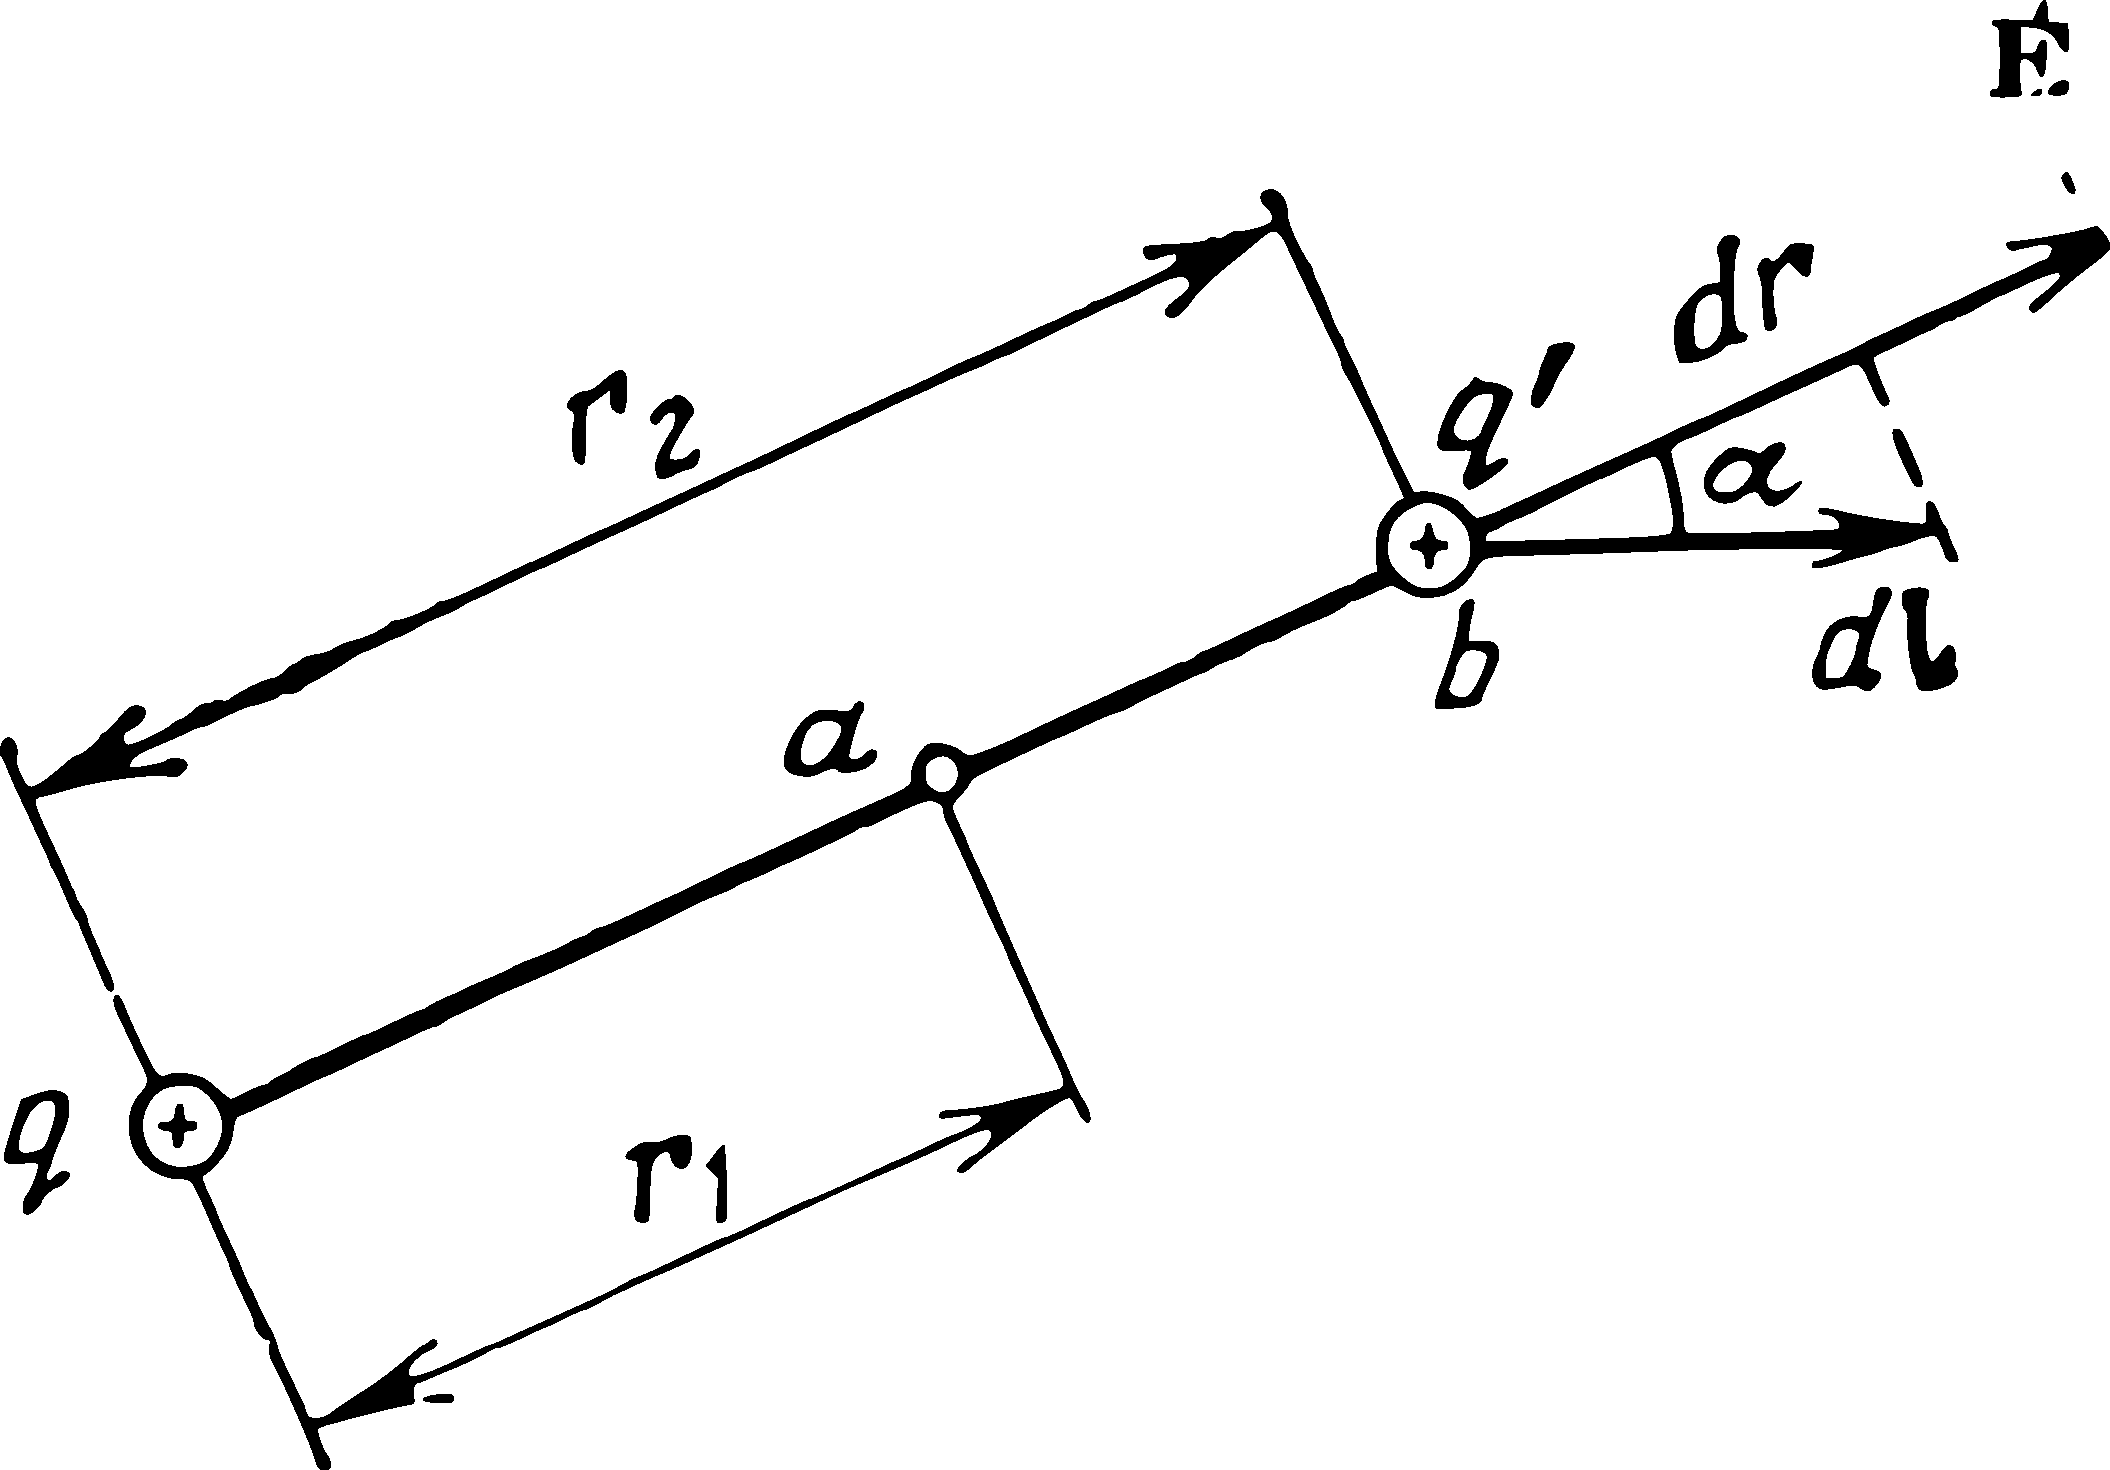
\includegraphics[width=\textwidth]{figs/ch-16/fig-16-01.pdf}
\caption{The work done in the movement of charge $q'$ from point $a$ to point $b$ in an electric field.\zhcap{电荷 $q'$ 在电场中从点 $a$ 移动到点 $b$ 时所做的功。}\label{fig-16-01}}
\end{marginfigure}
The work $W$ done by the electric forces of repulsion of like charges $q$ and $q'$ is positive when the-charges move away from each other, and negative when they move toward each other. The work done by electric forces of attraction of unlike charges ($q$ and $q'$ is positive when they move toward each other and negative when they move away from each other.
\zhpar{同号电荷 $q$ 与 $q'$ 之间静电斥力所做的功 $W$，当两电荷相互远离时为正，相互靠近时为负。异号电荷之间静电引力所做的功，当两电荷相互靠近时为正，相互远离时为负。}

\subsection{}\label{16.1.3} When an electric charge $q'$ is moved in a field set up by a system of point charges $q_{1}, \,q_{2}, \,\ldots{}, \,q_{n}$, the charge $q'$ is subject to the force
\zhpar{当电荷 $q'$ 处于由点电荷 $q_{1}, \,q_{2}, \,\ldots{}, \,q_{n}$ 产生的电场中移动时，电荷 $q'$ 受到的力为：}
\begin{equation*}%
\vb{F}= \vb{F}_{1} + \vb{F}_{2} + \ldots{} + \vb{F}_{n},
\end{equation*}
and the work $W$ done by the resultant force is equal to the algebraic sum of the work done by the component forces:
\zhpar{此时，作用于电荷 $q'$ 的合力所做的功 $W$ 等于各分力所做功的代数和：}
\begin{equation*}%
W = W_{1} + W_{2} + \ldots{} + W_{n} = \sum_{i=1}^{n} \frac{q_{i}q'}{4 \pi \epsilon_{0} \epsilon_{r}} \left( \frac{1}{r_{i1}} - \frac{1}{r_{i2}} \right),
\end{equation*}
where $r_{i2}$ and $r_{i2}$ are the distances of charge $q_{i}$ to the initial and final positions of charge $q'$. Each of the amounts of work $W_{i}$ and the total work $W$ depend upon the initial and final positions of the charge $q'$, but are independent of the shape of its path.
\zhpar{式中 $r_{i2}$ 与 $r_{i2}$ 分别为电荷 $q_{i}$ 到电荷 $q'$ 初始位置与终止位置的距离。各分功 $W_{i}$ 及总功 $W$ 都取决于电荷 $q'$ 的初始位置和终止位置，但与其路径的形状无关。}

\subsection{}\label{16.1.4} \redem{Circulation of the field strength vector} along the closed path or loop $L$ is the line integral
\zhpar{沿闭合路径或回路 $L$ 的\redem{场强矢量的环流}是如下的线积分：}
\begin{equation*}%
\oint_{L} E \, \dd l \cos \alpha = \oint_{L} \vb{E} \, \dd \vb{l}.
\end{equation*}
This integral is numerically equal to the work done by electrostatic forces in moving a unit positive charge along a closed path. Since $r_{i1} = r_{i2}$ for a closed path, we have, according to Sect. \ssect{16.1.3}, $\oint_{L} \vb{E} \, \dd \vb{l} = 0$, i.e. the above-mentioned work equals zero.
\zhpar{该积分在数值上等于静电力将单位正电荷沿闭合路径移动一周时所做的功。由于对闭合路径有 $r_{i1} = r_{i2}$，据\ssect{16.1.3}可得 $\oint_{L} \vb{E} \, \dd \vb{l} = 0$，即上述功为零。}

A force field of strength $\vb{E}$ that complies with such a condition is said to be a \redem{conservative one}. An electrostatic field is conservative.
\zhpar{满足这一条件的场强矢量 $\vb{E}$ 所对应的力场称为\redem{保守场}。静电场是保守场。}

The differential form of the condition indicating the conservative nature of an electrostatic field is one of Maxwell's equations for an electrostatic field \ssect{27.2.1}.
\zhpar{静电场保守性条件的微分形式，是静电场的麦克斯韦方程之一（\ssect{27.2.1}）。}


\section[Electrostatic Field Potential]{Potential of an Electrostatic Field}
\label{sec-16.2}
\zhtitle{静电场的电势}

\subsection{}\label{16.2.1} The work $\delta W$ \ssect{16.1.1} is equal to the decrease $\dd E_{p}$ in potential energy \ssect{3.3.1} of the charge $q'$ moving in an electrostatic field:
\zhpar{功 $\delta W$（\ssect{16.1.1}）等于在静电场中运动的电荷 $q'$ 的势能（\ssect{3.3.1}）的减少量 $\dd E_{p}$：}
\begin{equation*}%
\delta W = - \dd E_{p},
\end{equation*}
and
\zhpar{且}
\begin{equation*}%
W = \int_{a}^{b} q' E \dd l \cos \alpha =- \Delta E_{p} = E_{1P} - E_{2P},
\end{equation*}
where $E_{1P}$ and $E_{1P}$ are the values of the potential energy of
charge $q'$ at points $a$ and $b$, and $\alpha$ is the angle between the directions of vectors $\vb{E}$ and $\dd l$ (\figr{fig-16-01}).
\zhpar{式中 $E_{1P}$ 与 $E_{1P}$ 分别为电荷 $q'$ 在点 $a$ 与点 $b$ 处的势能值，$\alpha$ 为矢量 $\vb{E}$ 与 $\dd l$ 方向之间的夹角（见\figr{fig-16-01}）。}

\subsection{}\label{16.2.2} When point charge $q'$ is moved by electrostatic forces in a field set up by charge $q$, the change $\dd E_{p}$ in its potential energy in an infinitesimal displacement is
\zhpar{当点电荷 $q'$ 在由电荷 $q$ 产生的电场中受静电力作用而移动时，其势能在无穷小位移中的改变量 $\dd E_{p}$ 为：}
\begin{equation*}%
\dd E_{p} = -\delta W = - \frac{qq' \, \dd r}{4 \pi \varepsilon \varepsilon_{0} r^{2}}.
\end{equation*}
Upon a finite displacement of charge $q'$ from point $a$ to point $b$ (\figr{fig-16-01}), the change $\Delta E_{p}$ in the potential energy of the charge
is
\zhpar{当电荷 $q'$ 从点 $a$ 移动到点 $b$ 的有限位移中（见\figr{fig-16-01}），电荷势能的改变量 $\Delta E_{p}$ 为：}
\begin{align*}%
\Delta E_{p} & = E_{2p} - E_{1p} = \int_{r_{1}}^{r_{2}} \dd E_{p} \\
& = \frac{qq' \, \dd r}{4 \pi \varepsilon \varepsilon_{0} r_{2}} - \frac{qq' \, \dd r}{4 \pi \varepsilon \varepsilon_{0} r_{1}} && \text{(in SI units),} \\
\Delta E_{p} & =  qq'\left( \frac{1}{\varepsilon_{r} r_{2} - \varepsilon_{r} r_{1}} \right) && \text{(in CGSE units).}
\end{align*}

\subsection{}\label{16.2.3} When point charge $q'$ is moved in a field set up by a system of point charges $(q_{1},\, q_{2},\, \ldots , \, q_{n})$, the change in the potential energy of charge $q'$ is
\zhpar{当点电荷 $q'$ 在由点电荷系 $(q_{1},\, q_{2},\, \ldots , \, q_{n})$ 产生的电场中移动时，电荷 $q'$ 的势能改变量为：}
\begin{align*}%
\Delta E_{p} & =  q' \sum_{i = 1}^{n}\left( \frac{q_{i}}{4 \pi \varepsilon \varepsilon_{0} r_{i2}} - \frac{q_{i}}{4 \pi \varepsilon \varepsilon_{0} r_{i1}}\right) && \text{(in SI units)},\\
\Delta E_{p} & = q' \sum_{i = 1}^{n}\left( \frac{q_{i}}{\varepsilon_{r} r_{i2}} - \frac{q_{i}}{ \varepsilon_{r} r_{i1}}\right) && \text{(in CGSE units).}
\end{align*}
where $r_{i1}$ and $r_{i2}$ are the distances between charges $q_{i}$ and $q'$ before and after the displacement of the latter.
\zhpar{式中 $r_{i1}$ 与 $r_{i2}$ 分别为电荷 $q'$ 位移前、后与电荷 $q_{i}$ 之间的距离。}

\subsection{}\label{16.2.4} To find the absolute value of the potential energy of an electric charge at a given point of an electrostatic field, it is necessary to choose a reference point \ssect{3.3.4} for the potential energy. Integrating the equation in \ssect{16.2.2}, we obtain for the general case:
\zhpar{要求出静电场中某点处电荷势能的绝对值，必须为势能选定一个参考点（\ssect{3.3.4}）。对\ssect{16.2.2}中的方程积分，可得一般情形下：}
\begin{equation*}%
E_{p} = \frac{qq'}{4 \pi \varepsilon_{0} \varepsilon_{r} r} + C,
\end{equation*}
where $C$ is an arbitrary constant. If we assume that $E_{p} = 0$ as $r \to \infty$, then $C= 0$ and the potential energy of charge $q'$, located in the field of charge $q$ at the distance $r$ from this charge, equals
\zhpar{式中 $C$ 为任意常量。若假定当 $r \to \infty$ 时 $E_{p} = 0$，则 $C= 0$，位于电荷 $q$ 产生的电场中、距该电荷为 $r$ 处的电荷 $q'$ 的势能为：}
\begin{align*}%
E_{p} & = \frac{qq'}{4 \pi \varepsilon_{0} \varepsilon_{r} r}  && \text{(in SI units)},\\
E_{p} & = \frac{qq'}{\varepsilon_{r} r}   && \text{(in CGSE units.)}
\end{align*}
For like charges $q$ and $q'$ the potential energy of their inter­ action (repulsion) is positive and increases (decreases) as the charges move closer together (away from each other). In attraction of unlike charges $E_{p} < 0$ and increases to zero as one of the charges approaches infinity. The curves showing the dependence of the potential energy of two point charges on the distance between them are given in \figr{fig-16-02}.
\zhpar{对于同号电荷 $q$ 与 $q'$，其相互作用（斥力）的势能为正，并且随两电荷相互靠近而增大（随相互远离而减小）。异号电荷相互吸引时 $E_{p} < 0$，并且当其中一个电荷趋于无穷远时，$E_{p}$ 增大至零。两个点电荷的势能随二者间距离变化的曲线如\figr{fig-16-02}所示。}


\begin{marginfigure}[-2cm]
\centering
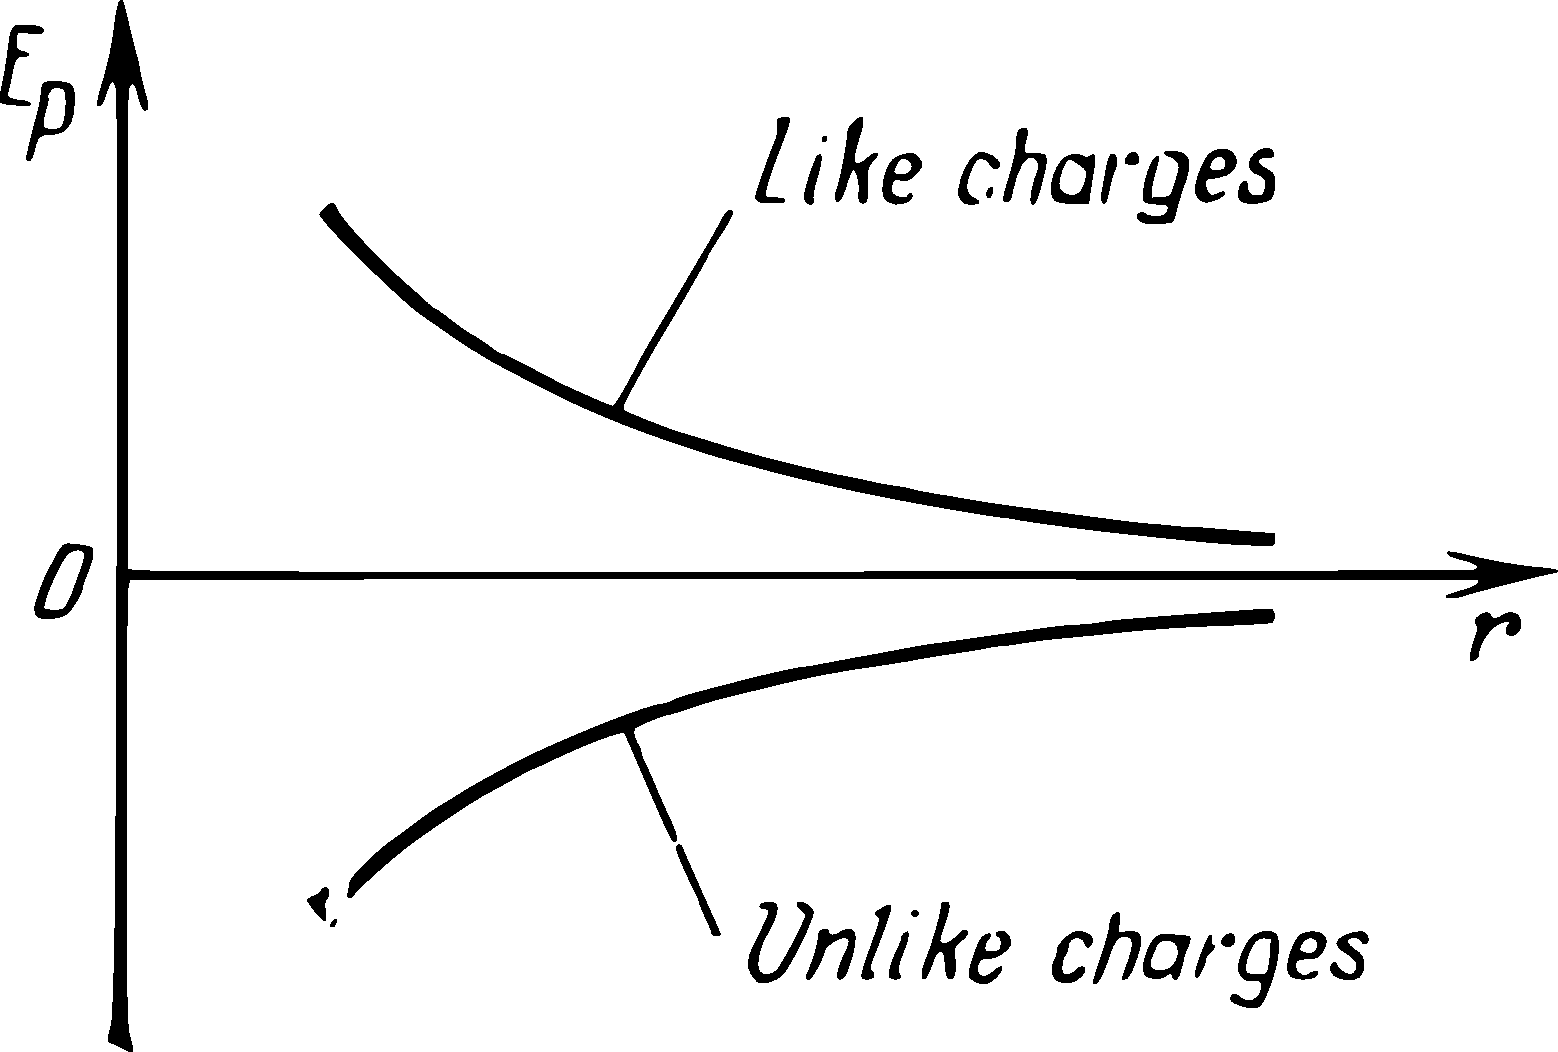
\includegraphics[width=\textwidth]{figs/ch-16/fig-16-02.pdf}
\caption{The dependence of the potential energy of two point charges on the distance between them.\zhcap{两个点电荷的势能随二者间距离的变化。}\label{fig-16-02}}
\end{marginfigure}


\subsection{}\label{16.2.5} The potential energy $E_{p}$ of charge $q'$, located in a field set up by a system of point charges $(q_{1},\, q_{2},\, \ldots , \, q_{n})$ is equal to the sum of the potential energies $E_{ip}$ in the fields set up by each of the charges separately:
\zhpar{位于点电荷系 $(q_{1},\, q_{2},\, \ldots , \, q_{n})$ 产生的电场中的电荷 $q'$ 的势能 $E_{p}$，等于每个电荷单独产生的电场中的势能 $E_{ip}$ 之和：}
\begin{equation*}%
E_{p} = \sum_{i=1}^{n} E_{ip} = q' \sum_{i=1}^{n} \frac{q_{i}}{4 \pi \varepsilon_{0} \varepsilon_{r} r_{i}} \quad \text{(in SI units.)}
\end{equation*}
where $r_{i}$ is the distance between charges $q_{i}$ and $q'$.
\zhpar{式中 $r_{i}$ 为电荷 $q_{i}$ 与电荷 $q'$ 之间的距离。}

\subsection{}\label{16.2.6} The \redem{potential of an electrostatic field} is an energy characteristic of the field, it is the ratio of the potential energy $E_{p}$ of charge $q'$ to the magnitude of the charge
\zhpar{\redem{静电场的电势}是表征电场能量性质的物理量，它等于电荷 $q'$ 的势能 $E_{p}$ 与该电荷电量之比：}
\begin{equation*}%
V = \frac{E_{p}}{q'} = \sum_{i = 1}^{n} \frac{q_{i}}{4 \varepsilon_{0} \varepsilon_{r} \pi r_{i}} \quad \text{(in SI units).}
\end{equation*}
This ratio is independent of the magnitude of the charge q' and is numerically equal to the potential energy of a unit test charge \ssect{15.1.3} placed at the point being considered in the field.
\zhpar{该比值与电荷 $q'$ 的大小无关，在数值上等于将单位试探电荷（\ssect{15.1.3}）置于场中所考虑的点时其所具有的势能。}

\hlblue{Examples.} 
\zhpar{\hlblue{例：}}
\begin{enumerate}[label=(\arabic*)]
\item The potential of an electrostatic field set up by one point charge $q$ in a homogeneous and isotropic dielectric is
\zhpar{由均匀各向同性电介质中单个点电荷 $q$ 产生的静电场的电势为：}
\begin{align*}%
V & = \frac{q}{4 \pi \varepsilon_{0} \varepsilon_{r} r} &&  \text{(in SI units),}\\
V & = \frac{q}{\varepsilon_{r} r} &&  \text{(in cgse units).}
\end{align*}

\item The potential of a field set up by a charged conductor \ssect{16.4.4} in a homogeneous and isotropic dielectric is
\zhpar{带电导体（\ssect{16.4.4}）在均匀各向同性电介质中产生的电场的电势为：}
\begin{align*}%
V & = \frac{1}{4 \pi \varepsilon_{0} \varepsilon_{r}} \oint_{S} \frac{\sigma \, \dd S}{r} &&  \text{(in SI units),}\\
V & = \frac{1}{\varepsilon_{r}} \oint_{S} \frac{\sigma \, \dd S}{r} &&  \text{(in cgse units).}
\end{align*}
where $\sigma$ is the surface charge density on the conductor \ssect{15.2.3} and $\dd S$ is an element of surface of the conductor.
\zhpar{式中 $\sigma$ 为导体表面的面电荷密度（\ssect{15.2.3}），$\dd S$ 为导体表面的面元。}

\item The potential of an isolated conducting sphere of radius $R$, having the charge $q$, is
\zhpar{半径为 $R$、带电荷量为 $q$ 的孤立导体球的电势为：}
\begin{align*}%
V & = \frac{q}{4 \pi \varepsilon_{0} \varepsilon_{r} R} &&  \text{(in SI units),}\\
V & = \frac{q}{\varepsilon_{r} R} &&  \text{(in cgse units).}
\end{align*}
\end{enumerate}

\subsection{}\label{16.2.7} The work $W$ done by electric forces in moving charge $q'$ from point $a$ to point $b$ of an electrostatic field is
\zhpar{静电力将电荷 $q'$ 从静电场中点 $a$ 移动到点 $b$ 时所做的功 $W$ 为：}
\begin{equation*}%
W = E_{1p} - E_{2p} = q'(V_{1} - V_{2}) = q' \Delta V,
\end{equation*}
where $E_{1p}$ and $E_{2p}$ are the potential energies of charge $q'$ at points $a$ and $b$, $V_{1}$ and $V_{2}$ are the potentials of the field at the same points, and $\Delta V = V_{1} - V_{2}$ is the \redem{potential difference}. If point $b$ is at infinity, $E_{2p} = 0$ and $V_{2} = 0$. Then the work $W_{\infty}$ required to move charge $q'$ from point a to infinity is equal to
\zhpar{式中 $E_{1p}$ 与 $E_{2p}$ 分别为电荷 $q'$ 在点 $a$ 与点 $b$ 处的势能，$V_{1}$ 与 $V_{2}$ 分别为电场在这两点的电势，$\Delta V = V_{1} - V_{2}$ 称为\redem{电势差}。若点 $b$ 位于无穷远处，则 $E_{2p} = 0$，$V_{2} = 0$。此时，将电荷 $q'$ 从点 $a$ 移至无穷远所需做的功 $W_{\infty}$ 为：}
\begin{equation*}%
W_{\infty} = E_{1p} = q' V_{1}.
\end{equation*}
Owing to the arbitrary nature of point $a$ subindex 1 can be discarded. Then
\zhpar{由于点 $a$ 的位置是任意选取的，下标 1 可以去掉。于是有}
\begin{equation*}%
V = \frac{W_{\infty}}{q}.
\end{equation*}
Hence, the potential at a given point of an electrostatic field is numerically equal to the work done by electrostatic forces in moving a unit positive charge from the point in the field to infinity. This work is also numerically equal to that done by external forces (acting against the forces of the electrostatic field) in moving a unit positive charge from infinity to the given point in the field.
\zhpar{因此，静电场中某点的电势在数值上等于静电力将单位正电荷从该点移至无穷远处所做的功。该功在数值上也等于外力（克服静电场力作用）将单位正电荷从无穷远处移至场中该点所做的功。}

\subsection{}\label{16.2.8} In the study of electrostatic fields, all the problems require a knowledge of the potential difference between any points in a field rather than the absolute values of the potentials at these points. Therefore, the choice of a point of zero potential depends only on its convenience for solving the given problem. It frequently proves convenient to assume that the potential of the earth is equal to zero.
\zhpar{在研究静电场时，所有问题所需要的都是场中任意两点之间的电势差，而不是这些点处电势的绝对值。因此，零电势点的选取只取决于求解具体问题时是否方便。通常假定大地的电势为零，这往往是很方便的。}


\section[Field Potential and Strength Relation]{Relation Between the Potential and Strength of an Electrostatic Field}
\label{sec-16.3}
\zhtitle{静电场的电势与场强的关系}

\subsection{}\label{16.3.1} On the basis of the equations in sections \ssect{16.2.1} and \ssect{16.2.6}, an element of work $\delta W$ done in the infinitesimal displacement of charge $q'$ in an electrostatic field is
\zhpar{根据\ssect{16.2.1}与\ssect{16.2.6}中的方程，静电场中电荷 $q'$ 在无穷小位移中所做的功元 $\delta W$ 为：}
\begin{align*}%
\delta W & = q' E \cos \alpha \dd l = - \dd E_{p} = -q' \, \dd V, \qor \\
E \cos \alpha \, \dd l & = - \dd V; \quad \vb{E}  \, \dd \vb{l} = - \dd V.
\end{align*}
But $\dd l \cos \alpha = \dd l_{0}$ where $\dd l_{0}$ is an element of length of the line of force \ssect{15.1.6} (\figr{fig-16-03}). Hence, $E = -\dv*{V}{l_{0}}$. The derivative $\dv{V}{l_{0}}$ is the rate of change of the potential along a line of force and is numerically equal to the change in potential per unit length of a line of force.
\zhpar{而 $\dd l \cos \alpha = \dd l_{0}$，其中 $\dd l_{0}$ 为电场线（\ssect{15.1.6}）的长度元（见\figr{fig-16-03}）。因此，$E = -\dv*{V}{l_{0}}$。导数 $\dv{V}{l_{0}}$ 为沿电场线方向电势的变化率，其数值等于沿电场线单位长度上的电势改变量。}

\begin{marginfigure}
\centering
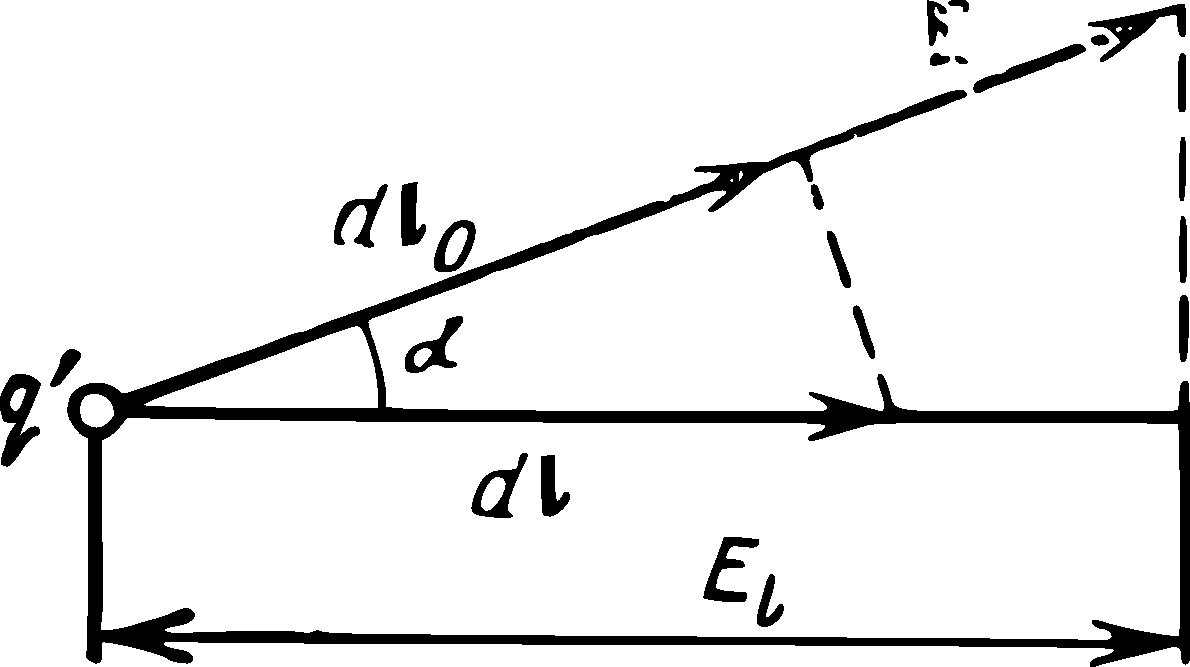
\includegraphics[width=\textwidth]{figs/ch-16/fig-16-03.pdf}
\caption{The field $E$ is numerically equal to the change in potential per unit length of a line of force.\zhcap{场强 $E$ 在数值上等于沿电场线方向单位长度上的电势变化。}\label{fig-16-03}}
\end{marginfigure}

\subsection{}\label{16.3.2} The projection $E_{l}$ of vector $\vb{E}$ on the direction of motion $\dd \vb{l}$ is equal to: $E_{l} = E \cos \alpha$. Therefore
\zhpar{矢量 $\vb{E}$ 在运动方向 $\dd \vb{l}$ 上的投影 $E_{l}$ 等于 $E_{l} = E \cos \alpha$。因此有}
\begin{equation*}
E_{l} = - \dv{V}{t}.
\end{equation*}
It is obvious that $E_{l} \leqslant E$ and $\abs{\dv*{V}{l}} \leqslant \abs{\dv*{V}{l_{0}}}$. Hence, $E_{l}$ and $\dv*{V}{l}$ reach their maximum values when $\dd \vb{l}$ is tangent to the line of force.
\zhpar{显然 $E_{l} \leqslant E$，且 $\abs{\dv*{V}{l}} \leqslant \abs{\dv*{V}{l_{0}}}$。因此，当 $\dd \vb{l}$ 与电场线相切时，$E_{l}$ 与 $\dv*{V}{l}$ 取得最大值。}

In the vicinity of a given point in an electrostatic field, the potential varies most rapidly in the direction of a line of force. The sense of vector $\vb{E}$ is toward the most rapid decrease in potential.
\zhpar{在静电场中某点附近，沿电场线方向电势的变化最快。矢量 $\vb{E}$ 的指向为电势降落最快的方向。}

\subsection{}\label{16.3.3}
In a more general form the relation between the strength and potential of an electrostatic field is
\zhpar{一般而言，静电场的场强与电势之间的关系为：}
\begin{equation*}%
\vb{E} = -\grad{V},
\end{equation*}
where $\grad{V}$ is the potential gradient vector, directed toward the most rapid increase in the potential and numerically equal to its rate of change per unit length in this direction. If the potential $V$ is regarded as a function of the three Cartesian coordinates of the given point in the field, then
\zhpar{式中 $\grad{V}$ 为电势梯度矢量，其方向指向电势增加最快的方向，其数值等于沿该方向单位长度上电势的变化率。若将电势 $V$ 视为场中给定点三个笛卡儿直角坐标的函数，则}
\begin{equation*}%
\grad{V} =\pdv{V}{x} \vu{i} + \pdv{V}{y} \vu{j} + \pdv{V}{z} \vu{k},
\end{equation*}
where $\vu{i}$, $\vu{j}$ and $\vu{k}$ are unit vectors along the $OX$, $OY$ and $OZ$ axes. The projections of the electrostatic field strength vector on the coordinate axes are related to the field potential by the equations:
\zhpar{式中 $\vu{i}$、$\vu{j}$ 与 $\vu{k}$ 分别为沿 $OX$、$OY$ 与 $OZ$ 轴的单位矢量。静电场场强矢量在坐标轴上的投影与场的电势之间由下列方程相联系：}
\begin{equation*}%
E_{x} = -\pdv{V}{x},\,\,E_{y} = -\pdv{V}{y},\,\,E_{z} = -\pdv{V}{z}.
\end{equation*}

\subsection{}\label{16.3.4}
 When an electric charge is moved in a direction $\dd \vb{l}$, perpendicular to a line of force, i.e. perpendicular to vector $\vb{E}$, $E_{l} = 0$ and $\dv*{V}{l} = 0$ \ssect{16.3.1}, i.e. $V = \text{const}$. The potential is the same at all points of a curve orthogonal to a line of force.
\zhpar{当电荷沿与电场线垂直（即与矢量 $\vb{E}$ 垂直）的方向 $\dd \vb{l}$ 移动时，$E_{l} = 0$，$\dv*{V}{l} = 0$（\ssect{16.3.1}），即 $V = \text{const}$。与电场线正交的曲线上所有点的电势都相同。}
 
The geometrical locus of all points having the same potential is called an \redem{equipotential surface}. It follows from the aforesaid that equipotential surfaces are everywhere orthogonal to lines of force.
\zhpar{具有相同电势的所有点的几何轨迹称为\redem{等势面}。由上述内容可知，等势面处处与电场线垂直。}

The work done in moving an electric charge along one and the same equipotential surface equals zero.
\zhpar{沿同一等势面移动电荷时所做的功等于零。}

An infinite number of equipotential surfaces can be constructed about any system of electric charges. They are usually constructed so that the potential difference is the same between any two adjacent equipotential surfaces.
\zhpar{对于任意一组电荷，都可以作出无穷多个等势面。通常作图时使任意两个相邻等势面之间的电势差相等。}

\subsection{}\label{16.3.5} There are two methods for the graphical representation of electrostatic fields: by means of lines of force and by means of equipotential surfaces. If the arrangement of the lines of force of an electrostatic field is known, equipotential surfaces can be constructed. Conversely, knowing the arrangement of the equipotential surfaces, the magnitude and direction of the field strength can be found for each point of the field, i.e. the lines of force can be constructed.
\zhpar{静电场的图示方法有两种：电场线法与等势面法。若已知静电场电场线的分布，即可作出等势面。反之，若已知等势面的分布，则可求出场中每一点处场强的大小与方向，从而作出电场线。}


\section{Conductors in an Electrostatic Field}
\label{sec-16.4}
\zhtitle{静电场中的导体}

\subsection{}\label{16.4.1} Solid metal conductors contain current carriers. These are conduction electrons (free electrons) that can be moved by the external electric field through the volume of the conductor. Conduction electrons appear when a conducting metal goes over from a less condensed to a more condensed state, i.e. from the gaseous to the liquid or solid state. At this valence electrons \ssect{39.3.9} are collectivized; they are separated from ``their'' atoms and form a special \redem{electron} gas.
\zhpar{金属导体中含有载流子。它们是传导电子（自由电子），在外部电场作用下可以穿过导体的整个体积移动。当导电金属由较稀疏的状态转变为较致密的状态，即由气态转变为液态或固态时，就会出现传导电子。此时，价电子（\ssect{39.3.9}）集体化，脱离“自身”的原子，形成一种特殊的\redem{电子气}。}

\subsection{}\label{16.4.2} The electrical properties of conductors under electrostatic conditions are determined by the behaviour of the conduction electrons in the external electrostatic field. In the absence of an external electrostatic field, the electric fields of the conduction electrons and the positive ions of the metal \ssect{40.1.3}, the atomic cores, mutually compensate each other. When a metal conductor is placed into an external electrostatic field, this field redistributes the conduction electrons in the conductor so that at any point within the conductor the conduction electrons and the positive ions compensate the external electrostatic field.
\zhpar{在静电条件下，导体的电学性质由传导电子在外部静电场中的行为决定。在没有外部静电场时，传导电子的电场与金属正离子（\ssect{40.1.3}）即原子实的电场相互抵消。当金属导体置于外部静电场中时，该电场使导体内的传导电子重新分布，使得导体内任一点处，传导电子与正离子的电场都能补偿外部静电场。}

At any point inside a conductor located in an electrostatic field, the strength of the resultant steady-state electric field is equal to zero.
\zhpar{处于静电场中的导体内部任一点，合成的稳恒电场强度都等于零。}

\subsection{}\label{16.4.3} At the surface of the conductor the field strength vector $\vb{E}$ should be normal to the surface. If this were not so the tangential component $\vb{E}_{\tau}$ of vector $\vb{E}$ would cause the charges to move along the conductor's surface, and this would contradict the fixed distribution of the charges. This leads to the following consequences:
\zhpar{导体表面上的场强矢量 $\vb{E}$ 应当与表面垂直。若非如此，矢量 $\vb{E}$ 的切向分量 $\vb{E}_{\tau}$ 将使电荷沿导体表面移动，这与电荷的固定分布相矛盾。由此得出以下结论：}
\begin{enumerate}[label=(\alph*)]
\item $\vb{E} = 0$ at all points inside the conductor; at all points on its surface $\vb{E} = \vb{E}_{n}$ (and $\vb{E}_{\tau} = 0$), where $\vb{E}_{n}$ is the normal component of the field strength vector;
\zhpar{导体内部所有点处 $\vb{E} = 0$；导体表面所有点处 $\vb{E} = \vb{E}_{n}$（且 $\vb{E}_{\tau} = 0$），其中 $\vb{E}_{n}$ 为场强矢量的法向分量；}
\item the whole volume of a conductor in an electrostatic field is equipotential, because, for any point within the conductor,
\zhpar{处于静电场中的导体，其整个体积都是等势的，因为对于导体内任一点，}
\begin{equation*}%
\dv{V}{l} = - E \cos \alpha = 0 \qand V = \text{const;}
\end{equation*}
\item the surface of the conductor is also equipotential \ssect{16.3.4}, because for any line on the surface
\zhpar{导体表面同样是等势面（\ssect{16.3.4}），因为对于表面上的任一条线，}
\begin{equation*}%
\dv{V}{l} = - E_{\tau} = 0 \qand V = \text{const;}
\end{equation*}
\item in a charged conductor the uncompensated charges are located only on its surface. This follows from the Ostrogradsky-Gauss electric flux theorem \ssect{15.3.3}, according to which the total charge $q$ inside a conductor and enclosed within a certain volume bounded by the arbitrary closed surface $S$ is equal to
\zhpar{带电导体中未被抵消的电荷只分布在其表面上。这可由奥斯特洛格拉茨基-高斯电通量定理（\ssect{15.3.3}）得出。根据该定理，导体内部由任意闭合曲面 $S$ 所包围的体积内的总电荷 $q$ 为：}
\begin{equation*}%
q = \Phi_{e} = \oint_{S} D \, \cos \alpha \, \dd S = 0,
\end{equation*}
because $D = 0$ at all points on the surface.
\zhpar{因为表面上所有点处 $D = 0$。}
\end{enumerate}

\subsection{}\label{16.4.4} When the electrostatic field is set up by a charged conductor the displacement and strength of this field close to the surface of the conductor are found by the equations
\zhpar{当带电导体产生静电场时，紧靠导体表面处的电位移与场强由下列方程给出：}
\begin{equation*}%
D_{n} = G \qand E_{n}= \frac{\sigma}{\varepsilon_{0}\varepsilon_{r}} \,\, \text{(in SI units)},
\end{equation*}
where $\vb{n}$ is the outward normal to the conductor's surface, $\sigma$ is the surface charge density \ssect{15.2.3}, $\varepsilon_{r}$ is the relative permittivity (dielectric constant) of the medium \ssect{14.2.4} and $\varepsilon_{0}$ is the electric constant in SI units \ssect{14.2.7}.
\zhpar{式中 $\vb{n}$ 为导体表面的外法线，$\sigma$ 为面电荷密度（\ssect{15.2.3}），$\varepsilon_{r}$ 为介质的相对电容率（亦称介电常量）（\ssect{14.2.4}），$\varepsilon_{0}$ 为 SI 制中的真空电容率（\ssect{14.2.7}）。}